\documentclass[submit,techrep]{ipsj}
%
\usepackage{amsmath,amssymb}
\usepackage{bm}
\usepackage[dvipdfmx]{graphicx}
\usepackage{ascmac}
\usepackage{latexsym}

\def\Underline{\setbox0\hbox\bgroup\let\\\endUnderline}
\def\endUnderline{\vphantom{y}\egroup\smash{\underline{\box0}}\\}
\def\|{\verb|}
\def\newblock{\hskip .11em plus .33em minus .07em}



\setcounter{巻数}{59}%vol53=2012
\setcounter{号数}{1}
\setcounter{page}{1}

\title {ウェブアプリ製品系列の UI プロトタイピング向け \\ プロダクトライン開発}
\etitle{Software Product Line Engineering for UI Prototyping of \\ a Web Application Family}

\affiliate{Kitakyu-u}{北九州市立大学}
\affiliate{Kyoto-u}{京都大学}

\author{山崎 進}{Yamazaki Susumu}{Kitakyu-u}[zacky@kitakyu-u.ac.jp]
\author{山田 麻里衣}{Yamada Marii}{Kitakyu-u}[x6mcb015@eng.kitakyu-u.ac.jp]
\author{高瀬 英希}{Takase Hideki}{Kyoto-u}[takase@i.kyoto-u.ac.jp]

\begin{abstract}
ウェブアプリやウェブサイトなどでプロトタイピングを行う場合,ユーザーインタフェース(UI)やコンテンツに複数のバリエーションが存在し,それらを比較・評価したいことがしばしばある。そこで,このようなバリエーションをもつプロトタイプを一種の製品系列であると捉え,ソフトウェアプロダクトラインを適用する試みを行った。具体的には,ウェブサイトのバリエーションをフィーチャーモデルとして記述し,我々が静的なウェブサイトのプラットフォームとして採用する Ruby ベースの Middleman において可変性を実現する仕組みを開発し,実際にウェブサイトのデザインと実装を行った。
\end{abstract}

\begin{jkeyword}
ソフトウェアプロダクトラインエンジニアリング, UIデザイン, ウェブアプリ開発, フィーチャーモデリング
\end{jkeyword}

\begin{eabstract}
Often, we develop prototypes of a web application or site, which has variation on user interface and contents, and then we want to compare and evaluate them. Thus, we regard such prototypes as a product line, and try to apply Software Product Line Engineering to them: we describe valiation of them as a feature model, develop a framework that realize it using Middleman based on Ruby that we adopt as a platform of a static web site, and design and implement them using it.
\end{eabstract}

\begin{ekeyword}
Software Product Line Engineering, UI Design, Web Application Development, Feature Modeling
\end{ekeyword}


\begin {document}
\maketitle

\section{はじめに}

ウェブアプリやウェブサイトなどでプロトタイピングを行う場合,ユーザーインタフェース(UI)やコンテンツに複数のバリエーションが存在し,それらを比較・評価したいことがしばしばある。たとえば,我々の開発したイベントのウェブサイトの事例\cite{SWEST}では,開発時点ではUIのバリエーションを複数比較したいという要望があり,かつイベントの進行とともにメニューやコンテンツに変化を設ける必要があった。

そこで,このようなバリエーションをもつプロトタイプを一種の製品系列であると捉え,ソフトウェアプロダクトライン\cite{SPLE}\cite{FORM}を適用する試みを行った。具体的には,ウェブサイトのバリエーションをフィーチャーモデル\cite{FORM}として記述してみることを試みた。

本研究の目的は,ウェブアプリやウェブサイトのプロトタイピングで,UIやコンテンツのバリエーションを記述し,そのバリエーションの選択肢を与えてプレビューを表示したり,全てのバリエーションの組み合わせを一括でプレビューを表示したりするような静的ウェブページ構築の方法を提案することである。

アプローチは次のとおりである。

\begin{enumerate}
 \item バリエーションを記述する方法としてフィーチャーモデル\cite{FORM}を用いる。
 \item 静的ウェブページの構築の手段としてはMiddleman\cite{Middleman}を用いる。Middlemanを用いてバリエーションの選択肢を与えたり,全てのバリエーションの組み合わせを一括で表示できたりするようにする。
\end{enumerate}

\section{研究の動機となった開発事例について}

SWEST\cite{SWEST}では2017年から高瀬と山崎の手によりウェブサイトのリニューアルに着手した。高瀬がWordPressによるデザインと実装を行い,山崎がRubyスクリプトによるプログラムページのデザインと実装を行って,これらを併用することによって公開に至った。プログラムページのデザインには山田も部分的に加わり,配色などを検討した。

イベント終了後に山崎が報告ページの開発を行った。Middleman\cite{Middleman} を採用することで,その高い記述性と再利用性により,たった数日程度の短期間で開発することができた。2018年2月時点で\cite{SWEST}にて公開されているウェブページは,この段階のものである。

この経験を踏まえて,2018年からMiddlemanを全面的に採用したウェブサイトのリニューアルを行うことを企画した。現在,開発中であり,2018年3月のキックオフには公開する予定である。このデザインリニューアルでは,SWESTプログラム委員長の高瀬から,山田と山崎が要望のヒアリングを行い,山田が主にデザインを,山崎が主にMiddlemanによる実装を行う。

デザインについては,単に意匠のデザインを行っただけでなく,情報デザイン(たとえば\cite{InfoDesign}\cite{InfoDesignWorkshop})を行った。すなわち,ヒアリング内容を元に,ウェブサイトで開示する情報を読み手にどのように伝えると効果的かについて分析を行ってからデザインを行った。



\section{デザインプロセスの進行とフィーチャーモデルの変化}

本事例でフィーチャーモデルを導入した理由は,ヒアリングの結果,UIに関して実際にデザイン・実装して評価したいデザイン候補案が複数挙がったためである。ペーパープロトタイプでは良し悪しの判断がつかず,実際にデザイン・実装をして,ユーザビリティを評価してみないと,どの選択肢を採用したらいいかが判断できなかった。

また,複数の選択肢が要望として挙がってきたが,これらの選択肢をきちんと明文化する必要があり,かつ土曜な組み合わせが存在するのか,またそれらを網羅的に検討する必要性があった。

そこで,これを一種のプロダクトライン\cite{SPLE}\cite{FORM}だとみなし,可変性をフィーチャーモデル\cite{FORM}で表現することで,明確に要望を定義しようとした。

最初にモデル化したフィーチャーモデルは図\ref{fig:SWEST-FM-1}である。たとえば,サブメニューについて,「つける」もしくは「つけない」のどちらかを選択するという,択一(alternative)のフィーチャーが存在する,というような意味合いである。ここで,「募集の位置」「募集の表示時期」「サブメニュー」のような選択的なフィーチャーのことを可変点と呼ぶ。フィーチャーモデルは,どのようなバリエーションがあるか,すなわち可変性を明文化することができる。フィーチャーモデルを採用することで,可変性を明文化することができ,組み合わせを網羅的に検討することができる。

\begin{figure}[tb]
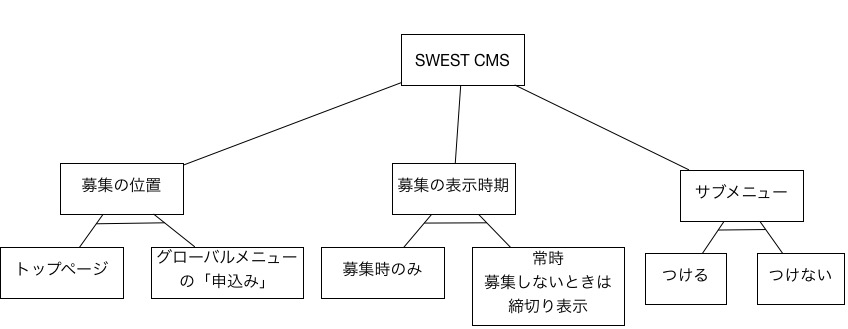
\includegraphics[width=80mm]{SWEST-feature-model-1.jpg}
\caption{フィーチャーモデル(1)}
\ecaption{The Feature Model (1)}
\label{fig:SWEST-FM-1}
\end{figure}

これを基に再度ヒアリングを進めたところ,さらに他のUIの可変性が明らかになり,さらに可変性としてはイベントの進行に伴って現れる可変性もあることが明らかになった。そのフィーチャーモデルは図\ref{fig:SWEST-FM-2}である。

\begin{figure*}[tb]
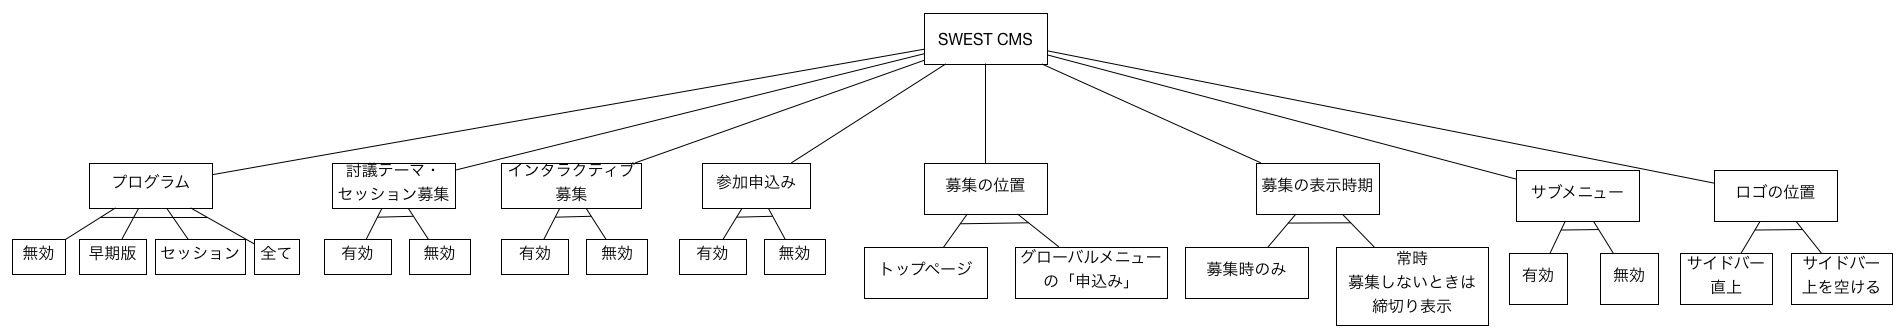
\includegraphics[width=170mm]{SWEST-feature-model-2.jpg}
\caption{フィーチャーモデル(2)}
\ecaption{The Feature Model (2)}
\label{fig:SWEST-FM-2}
\end{figure*}

当初このままMiddlemanにて実装を行い,全ての可変性の候補の組み合わせをプレビューするウェブサイトの構築を行おうとした。一般に,可変点を削減することで,組み合わせの数を減らすことができる。

この段階でデザインの検討を進めたことで,可変点のうちの1つ「募集の位置」を削減することにした。この可変点は,参加募集・テーマ募集・インタラクティブセッション募集の3つ存在する募集ページについて,メニューを設けずにトップページに集約する方式と,グローバルメニューにそれぞれの募集メニューを表示する方式の2つのUIのバリエーションを比較検討するというものであった。デザインの検討を進めたことで,次のような理由でグローバルメニューにそれぞれの募集メニューを表示する方式の方が妥当であると判断したため,可変点にはせず固定にすることにした。

\begin{enumerate}
  \item それぞれの募集に関して,記述する内容が多い。現代においては,スマートフォンでの表示を最大限考慮してデザインする必要がある。もしトップページに各募集ページを羅列するようにデザインすると,スマートフォンで表示した時に長大なコンテンツを表示することとなり,扱いにくくなる。
  \item 他のページはグローバルメニューから個別のページへ遷移するようにデザインされている。もしトップページにそれぞれの募集についての記述を書いた場合には,メニューから1クリックで遷移できるようにするためにはトップページのサブメニューに各募集ページを掲載する必要がある。このようにすると,トップページのみサブメニューが存在することになり,他のページとルールが異なるので,ユーザーが混乱する懸念がある。
\end{enumerate}

この点を踏まえて更新したフィーチャーモデルは図\ref{fig:SWEST-FM-3}である。これにより,可変点が7つ存在することが明らかになった。これらのうち「プログラム」「討議テーマ・セッション募集」「インタラクティブ募集」「参加申込み」がイベントの進行とともに現れるコンテンツのバリエーションを表し,「募集の表示時期」「サブメニュー」「ロゴの位置」がUIのバリエーションを表す。

「プログラム」の可変点については,バリエーションが4通りある。それ以外の可変点では,バリエーションがそれぞれ2通りある。全ての組み合わせは,256通り存在することが明らかになった。このうちUIのバリエーションについては,8通りの組み合わせがある。

\begin{figure*}[tb]
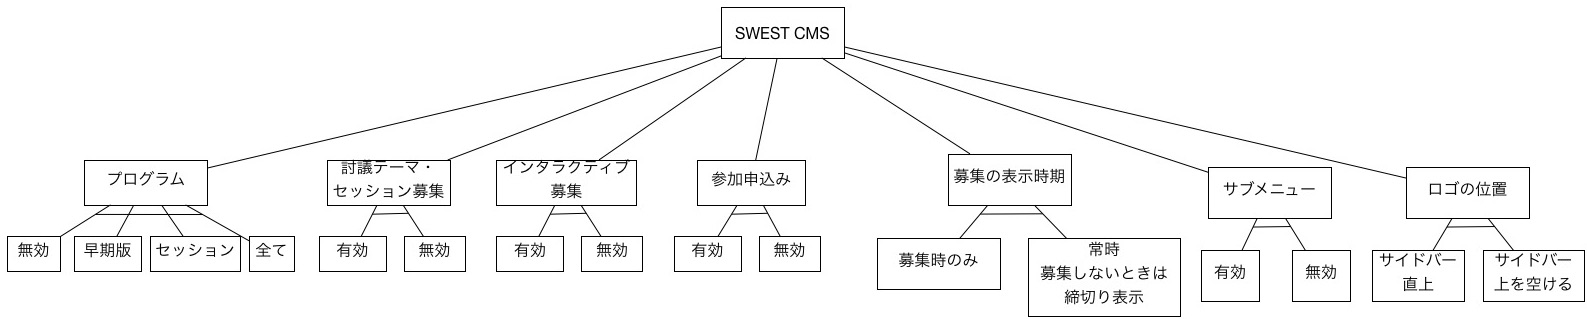
\includegraphics[width=170mm]{SWEST-feature-model-3.jpg}
\caption{フィーチャーモデル(3)}
\ecaption{The Feature Model (3)}
\label{fig:SWEST-FM-3}
\end{figure*}

\section{実装}

デザインの実装にはMiddleman\cite{Middleman}を用いた。まず,フィーチャーモデルに現れる各フィーチャーをオプション変数として設定を与えることで,可変性をオプションに与えた通りに設定してプレビューと本番サイトを生成するスクリプトを開発した。

次に,考えられる全ての組み合わせを静的に生成し,URLの一部にオプションを記述することでバリエーションを選択するようなプレビューを生成するスクリプトを開発した。この全ての組み合わせを含むプレビューをプロトタイプとして顧客や想定ユーザーに提示することで,どのバリエーションが意図に近いあるいは利用しやすいかを評価する。

ただし,全ての組み合わせ(256通り)を生成すると時間がかかるため,今回はUIのバリエーション(8通り)のみの組み合わせを表示することに絞った。

今回のフィーチャーモデルでは,択一(alternative)のフィーチャーしか現れなかったため,全ての組み合わせを網羅することが可能であった。もし任意(optional)のフィーチャー,すなわち存在したりしなかったりを選択できるフィーチャーや,要求(require)のフィーチャー,すなわちあるフィーチャーを選択した場合,別のフィーチャーを必要とするような関係性が現れたとしても,組み合わせを網羅することは可能であろう。

ただし,容量などのパラメータの選択肢を与えるフィーチャーが含まれる場合には,代表的な選択肢をあげることで,択一のフィーチャーに変換してやる必要がある。

\section{まとめと将来課題}

UIやコンテンツに複数のバリエーションを持つウェブアプリやウェブサイトにて,フィーチャーモデル\cite{FORM}を用いてバリエーションを記述することで,UIやコンテンツのバリエーションを明確にかつ簡潔に記述することができた。

次に,我々が静的なウェブサイトのプラットフォームとして採用する Ruby ベースの Middleman \cite{Middleman}において可変性を実現する仕組みを開発し,実際にウェブサイトのデザインと実装を行った。これにより,フィーチャーモデルで記述したバリエーションと同じ抽象レベルで,どの選択肢を選択するかオプションを指定することで,ウェブサイトの設定を簡潔に指定することができるようになった。また,プレビュー画面にて,全ての可能な選択肢を静的に生成することで,UIの比較検討を行いやすくすることができた。

将来課題としては,このような仕組みを再利用しやすくするために,Middleman のカスタム拡張\cite{Middleman}を開発し公開することが挙げられる。


\section*{謝辞}

SWEST実行委員のみなさまには特に感謝します。また,ウェブサイトの開発にあたり多大な助言をくださった parcel チームの Devon Govett と Shawn Presser にも感謝します。


\bibliographystyle{ipsjsort}
\bibliography{reference}

\end{document}
